% Options for packages loaded elsewhere
\PassOptionsToPackage{unicode}{hyperref}
\PassOptionsToPackage{hyphens}{url}
\PassOptionsToPackage{dvipsnames,svgnames,x11names}{xcolor}
%

\documentclass[
  10pt,
  letterpaper,
  a4paper, twoside]{scrreprt}
% \documentclass[twoside, fontsize=10pt]{scrreport}
\usepackage{amsmath,amssymb}
\usepackage{iftex}
\ifPDFTeX
  \usepackage[T1]{fontenc}
  \usepackage[utf8]{inputenc}
  \usepackage{textcomp} % provide euro and other symbols
\else % if luatex or xetex
  \usepackage{unicode-math}
  \defaultfontfeatures{Scale=MatchLowercase}
  \defaultfontfeatures[\rmfamily]{Ligatures=TeX,Scale=1}
\fi
% Use upquote if available, for straight quotes in verbatim environments
\IfFileExists{upquote.sty}{\usepackage{upquote}}{}
\usepackage{xcolor}

\usepackage[top=30mm,left=20mm,lmargin=30mm,,textwidth =
15.5cm,,textheight = 22.5cm]{geometry}

\usepackage{pdflscape}

\setlength{\emergencystretch}{3em} % prevent overfull lines
\setcounter{secnumdepth}{5}
% Make \paragraph and \subparagraph free-standing
\ifx\paragraph\undefined\else
  \let\oldparagraph\paragraph
  \renewcommand{\paragraph}[1]{\oldparagraph{#1}\mbox{}}
\fi
\ifx\subparagraph\undefined\else
  \let\oldsubparagraph\subparagraph
  \renewcommand{\subparagraph}[1]{\oldsubparagraph{#1}\mbox{}}
\fi



\providecommand{\tightlist}{%
  \setlength{\itemsep}{0pt}\setlength{\parskip}{0pt}}\usepackage{longtable,booktabs,array}
\usepackage{calc} % for calculating minipage widths
% Correct order of tables after \paragraph or \subparagraph
\usepackage{etoolbox}
\makeatletter
\patchcmd\longtable{\par}{\if@noskipsec\mbox{}\fi\par}{}{}
\makeatother
% Allow footnotes in longtable head/foot
\IfFileExists{footnotehyper.sty}{\usepackage{footnotehyper}}{\usepackage{footnote}}
\makesavenoteenv{longtable}
\usepackage{graphicx}
\makeatletter
\def\maxwidth{\ifdim\Gin@nat@width>\linewidth\linewidth\else\Gin@nat@width\fi}
\def\maxheight{\ifdim\Gin@nat@height>\textheight\textheight\else\Gin@nat@height\fi}
\makeatother
% Scale images if necessary, so that they will not overflow the page
% margins by default, and it is still possible to overwrite the defaults
% using explicit options in \includegraphics[width, height, ...]{}
\setkeys{Gin}{width=\maxwidth,height=\maxheight,keepaspectratio}
% Set default figure placement to htbp
\makeatletter
\def\fps@figure{htbp}
\makeatother

\usepackage{scrlayer-scrpage}
\automark[section]{section}
\cfoot[]{EKMF} 
\ifoot[]{Fretwurst}
\ofoot[]{\pagemark}
\usepackage{hyperref}
\usepackage[ngerman]{varioref}
\usepackage[ngerman]{cleveref}
\usepackage{eso-pic}
\usepackage[german=swiss]{csquotes}
\usepackage{pdfpages}
\usepackage[skip = 12pt, font=large,labelfont={large}]{caption}
\usepackage{float}
\usepackage{makecell}
\makeatletter
\@ifpackageloaded{tcolorbox}{}{\usepackage[skins,breakable]{tcolorbox}}
\@ifpackageloaded{fontawesome5}{}{\usepackage{fontawesome5}}
\definecolor{quarto-callout-color}{HTML}{909090}
\definecolor{quarto-callout-note-color}{HTML}{0758E5}
\definecolor{quarto-callout-important-color}{HTML}{CC1914}
\definecolor{quarto-callout-warning-color}{HTML}{EB9113}
\definecolor{quarto-callout-tip-color}{HTML}{00A047}
\definecolor{quarto-callout-caution-color}{HTML}{FC5300}
\definecolor{quarto-callout-color-frame}{HTML}{acacac}
\definecolor{quarto-callout-note-color-frame}{HTML}{4582ec}
\definecolor{quarto-callout-important-color-frame}{HTML}{d9534f}
\definecolor{quarto-callout-warning-color-frame}{HTML}{f0ad4e}
\definecolor{quarto-callout-tip-color-frame}{HTML}{02b875}
\definecolor{quarto-callout-caution-color-frame}{HTML}{fd7e14}
\makeatother
\makeatletter
\@ifpackageloaded{bookmark}{}{\usepackage{bookmark}}
\makeatother
\makeatletter
\@ifpackageloaded{caption}{}{\usepackage{caption}}
\AtBeginDocument{%
\ifdefined\contentsname
  \renewcommand*\contentsname{Inhaltsverzeichnis}
\else
  \newcommand\contentsname{Inhaltsverzeichnis}
\fi
\ifdefined\listfigurename
  \renewcommand*\listfigurename{Abbildungsverzeichnis}
\else
  \newcommand\listfigurename{Abbildungsverzeichnis}
\fi
\ifdefined\listtablename
  \renewcommand*\listtablename{Tabellenverzeichnis}
\else
  \newcommand\listtablename{Tabellenverzeichnis}
\fi
\ifdefined\figurename
  \renewcommand*\figurename{Abbildung}
\else
  \newcommand\figurename{Abbildung}
\fi
\ifdefined\tablename
  \renewcommand*\tablename{Tabelle}
\else
  \newcommand\tablename{Tabelle}
\fi
}
\@ifpackageloaded{float}{}{\usepackage{float}}
\floatstyle{ruled}
\@ifundefined{c@chapter}{\newfloat{codelisting}{h}{lop}}{\newfloat{codelisting}{h}{lop}[chapter]}
\floatname{codelisting}{Listing}
\newcommand*\listoflistings{\listof{codelisting}{Listingverzeichnis}}
\makeatother
\makeatletter
\makeatother
\makeatletter
\@ifpackageloaded{caption}{}{\usepackage{caption}}
\@ifpackageloaded{subcaption}{}{\usepackage{subcaption}}
\makeatother
\makeatletter
\@ifpackageloaded{sidenotes}{}{\usepackage{sidenotes}}
\@ifpackageloaded{marginnote}{}{\usepackage{marginnote}}
\makeatother
\ifLuaTeX
\usepackage[bidi=basic]{babel}
\else
\usepackage[bidi=default]{babel}
\fi
\babelprovide[main,import]{nswissgerman}
% get rid of language-specific shorthands (see #6817):
\let\LanguageShortHands\languageshorthands
\def\languageshorthands#1{}
\ifLuaTeX
  \usepackage{selnolig}  % disable illegal ligatures
\fi
\usepackage{csquotes}
\IfFileExists{bookmark.sty}{\usepackage{bookmark}}{\usepackage{hyperref}}
\IfFileExists{xurl.sty}{\usepackage{xurl}}{} % add URL line breaks if available
\urlstyle{same} % disable monospaced font for URLs


\hypersetup{
 pdflang = de, colorlinks = true, linkcolor = black, urlcolor = black,
 pdfauthor={ , Stefanie },
    pdfsubject={Absolvierendenbefragung des BfS für das IKMZ},
    pdftitle={Absolvierendenbefragung des BfS für das IKMZ},
    pdfkeywords={Befragung, Absolvierende, Alumni, IKMZ, Kommunikationswissenschaft}
   lang = {DE}
}

\usepackage{scrlayer-scrpage}

\definecolor{headergray}{RGB}{192,192,192}

\addtokomafont{disposition}{\sffamily}
\renewcommand{\familydefault}{\sfdefault}

\title{}
\date{}

\setlength{\abovecaptionskip}{10pt plus 3pt minus 2pt}
\setlength{\belowcaptionskip}{12pt plus 3pt minus 2pt}

\captionsetup{justification=raggedright, singlelinecheck=false}

%%%%%%%%%%%%%%%%%%%%%%%%%%%%%%%%%%%%%%%%%%%%

              %Dokumentstart

%%%%%%%%%%%%%%%%%%%%%%%%%%%%%%%%%%%%%%%%%%%%


\begin{document}

\pagestyle{scrheadings}
\clearscrheadfoot
\ohead{\textcolor{headergray}{\pagemark}}

\automark[section]{chapter}
\ihead{\textcolor{headergray}{\headmark}}

\ofoot{}
\ifoot{}

%\cfoot[]{Einführung in die Kommunikationswissenschaft und
Medienforschung -- EKMF} %unten Mitte
%\setheadsepline{.2pt}



\begin{titlepage}
\sffamily

\setlength\parindent{0pt}

\hfill 
\includegraphics[width = 6cm]{files/LaTeX/uzh_logo_d_pos.pdf}\par

\vspace{2cm}


{\bfseries\Huge Einführung in die Kommunikationswissenschaft und
Medienforschung --
EKMF \\[1cm] } % Den Zeilenumbruch immer ins Huge mit rein, damit der Zeilenabstand auch angepasst wird

 {\bfseries\Large Begleittext zum Modul (254-001a) \\[1cm]} 

{\bfseries \Large
 Stefanie Hangartner  \\ [1cm]
}


 
\vfill
{\bfseries \Large Version 0.01  \\[1cm] } 


\vfill 

Zuletzt aktualisiert: 2024-03-26

\vfill

\begin{tabbing}
Kontakt:\\
Dr. Benjamin Fretwurst\\
Institut für Kommunikationswissenschaft und Medienforschung -- IKMZ\\
Andreasstrasse 15\\
8050 Zürich\\
b.fretwurst@ikmz.ch\\[0.3cm]
\end{tabbing}

\setlength\parindent{1em}

\end{titlepage}

\makeatletter
\AddToShipoutPicture{\setlength{\unitlength}{1cm}\put(24.32,18.65){{
\includegraphics[height=.6cm]{files/LaTeX/uzh_logo_d_pos.pdf}}}}
\makeatletter

\cleardoublepage

%Überschriften unterdrücken durch IV und TV (wegen multicolumn)
\renewcommand{\listoftables}{\@starttoc{lot}}
\renewcommand{\tableofcontents}{\@starttoc{toc}}
\renewcommand{\listoffigures}{\@starttoc{lof}}

%Mehr Platz für breite Tabellennummern
\renewcommand{\l@table}{\@dottedtocline{1}{1em}{3em}}
\makeatother

\section*{Inhalt}
\label{sec:inhalt}
\pdfbookmark[1]{\contentsname}{toc}
%  \begin{multicols}{2}
    \tableofcontents
%  \end{multicols}


% \pdfbookmark[1]{Tabellen/Abbildungen}{lot}
\subsection*{Tabellenverzeichnis}
\label{sec:tabellenverzeichnis}

%\begin{multicols}{2}
\listoftables
%\end{multicols}

\subsection*{Abbildungsverzeichnis}
\label{sec:Abbildungsverzeichnis}

%\begin{multicols}{2}
\listoffigures
%\end{multicols}

\clearpage

% \maketitle

% 

\renewcommand{\familydefault}{\sfdefault}

\setlength{\parindent}{1em}

\bookmarksetup{startatroot}

\chapter*{Einleitung und Syllabus}\label{einleitung-und-syllabus}
\addcontentsline{toc}{chapter}{Einleitung und Syllabus}

\markboth{Einleitung und Syllabus}{Einleitung und Syllabus}

\section*{Syllabus}\label{syllabus}
\addcontentsline{toc}{section}{Syllabus}

\markright{Syllabus}

\section*{Vorwort}\label{vorwort}
\addcontentsline{toc}{section}{Vorwort}

\markright{Vorwort}

Sicher freuen Sie sich schon auf \enquote{Statistik: Aufbau}, und ich
glaube, Sie haben allen Grund dazu. Manche freuen sich weniger -- was ja
auch normal und ok ist. Wieder andere, denken lieber daran, wie das
Leben so sein wird, wenn Sie \enquote{Statistik: Aufbau} hinter sich
haben. Ihnen allen soll dieser Begleittext zur Seite stehen, damit Sie
aus dem Modul das für sich Beste rausholen. Diejenigen, die in der
Statistik ein mächtiges Tool entdecken, will ich ein tiefergehendes
Verständnis ermöglichen. Denen, die die Statistik einfach gut
absolvieren wollen, soll das Wichtigste vermittelt werden und die mit
Graus auf das Modul schauen, soll das Grauen genommen und etwas
Greifbares und Handhabbares angeboten werden, das sich -- mit zumutbaren
Investitionen -- lösen lässt. Hier in der Einleitung schreibe ich Ihnen,
was ich über den Sinn und die Mächtigkeit von Statistik denke sowie die
möglichen Ursachen für das Unbehagen denke.\\
\noindent Liebe Grüsse\\
Benjamin Fretwurst

\section*{Was bringt uns Statistik}\label{was-bringt-uns-statistik}
\addcontentsline{toc}{section}{Was bringt uns Statistik}

\markright{Was bringt uns Statistik}

Unser Alltag ist von Beobachtungen geprägt, aus denen wir etwas über uns
und die Welt lernen. Wir stellen Vermutungen an und haben das Gefühl,
dass wir wissen, wie es läuft. Das heisst, wir machen viele
Beobachtungen und ziehen unsere Schlüsse daraus. Wir entwickeln also aus
empirischen Beobachtungen Theorien. Diese Beobachtungen sind nur nicht
sehr systematisch und die Schlüsse, die wir aus ihnen ziehen sind mal
mehr von einer Erinnerung und mal mehr von einer anderen Erinnerung
geprägt. Wenn wir an dieses Erfahrungswissen etwas wissenschaftlicher
herangehen wollen, um systematisch Erkenntnisse zu erlangen, auf die wir
uns besser verlassen können, dann machen wir emprische Forschung.

blabla

\begin{center}\rule{0.5\linewidth}{0.5pt}\end{center}

\textbf{Was beschreibt die Funktion von Statistik am besten?}

Versuchen Sie es mit Ihren eigenen Worten.

\begin{center}\rule{0.5\linewidth}{0.5pt}\end{center}

\section*{Überblick Analysemethoden}\label{uxfcberblick-analysemethoden}
\addcontentsline{toc}{section}{Überblick Analysemethoden}

\markright{Überblick Analysemethoden}

Der folgende Überblick zeigt die statistischen Verfahren, mit deren
Hilfe kausale Zusammenhänge, Unterschiede und Datengruppierungen
analysiert werden können. Diese verschiedenen Analysemethoden
ermöglichen es, Daten aus unterschiedlichen Blickwinkeln zu analysieren.
Man kann also mit denselben Variablen eine Zusammenhangsanalyse machen
oder sie auf Unterschiede hin analysieren oder schauen, ob es
Interdependenzen gibt, sie als Gruppen bilden. Die zugrundeliegenden
Beziehungen in den Daten sind natürlich immer dieselben. Das liegt
daran, dass Unterschiede durch Zusammenhänge entstehen und Zusammenhänge
aufgrund von Unterschieden. Beides finden seine Ursache darin, dass
Variablen und Fälle Gruppen bilden; und gleichzeitig entstehen die
Gruppen durch die Zusammenhänge und Unterschiede.

blabla

\begin{figure}[H]

{\centering 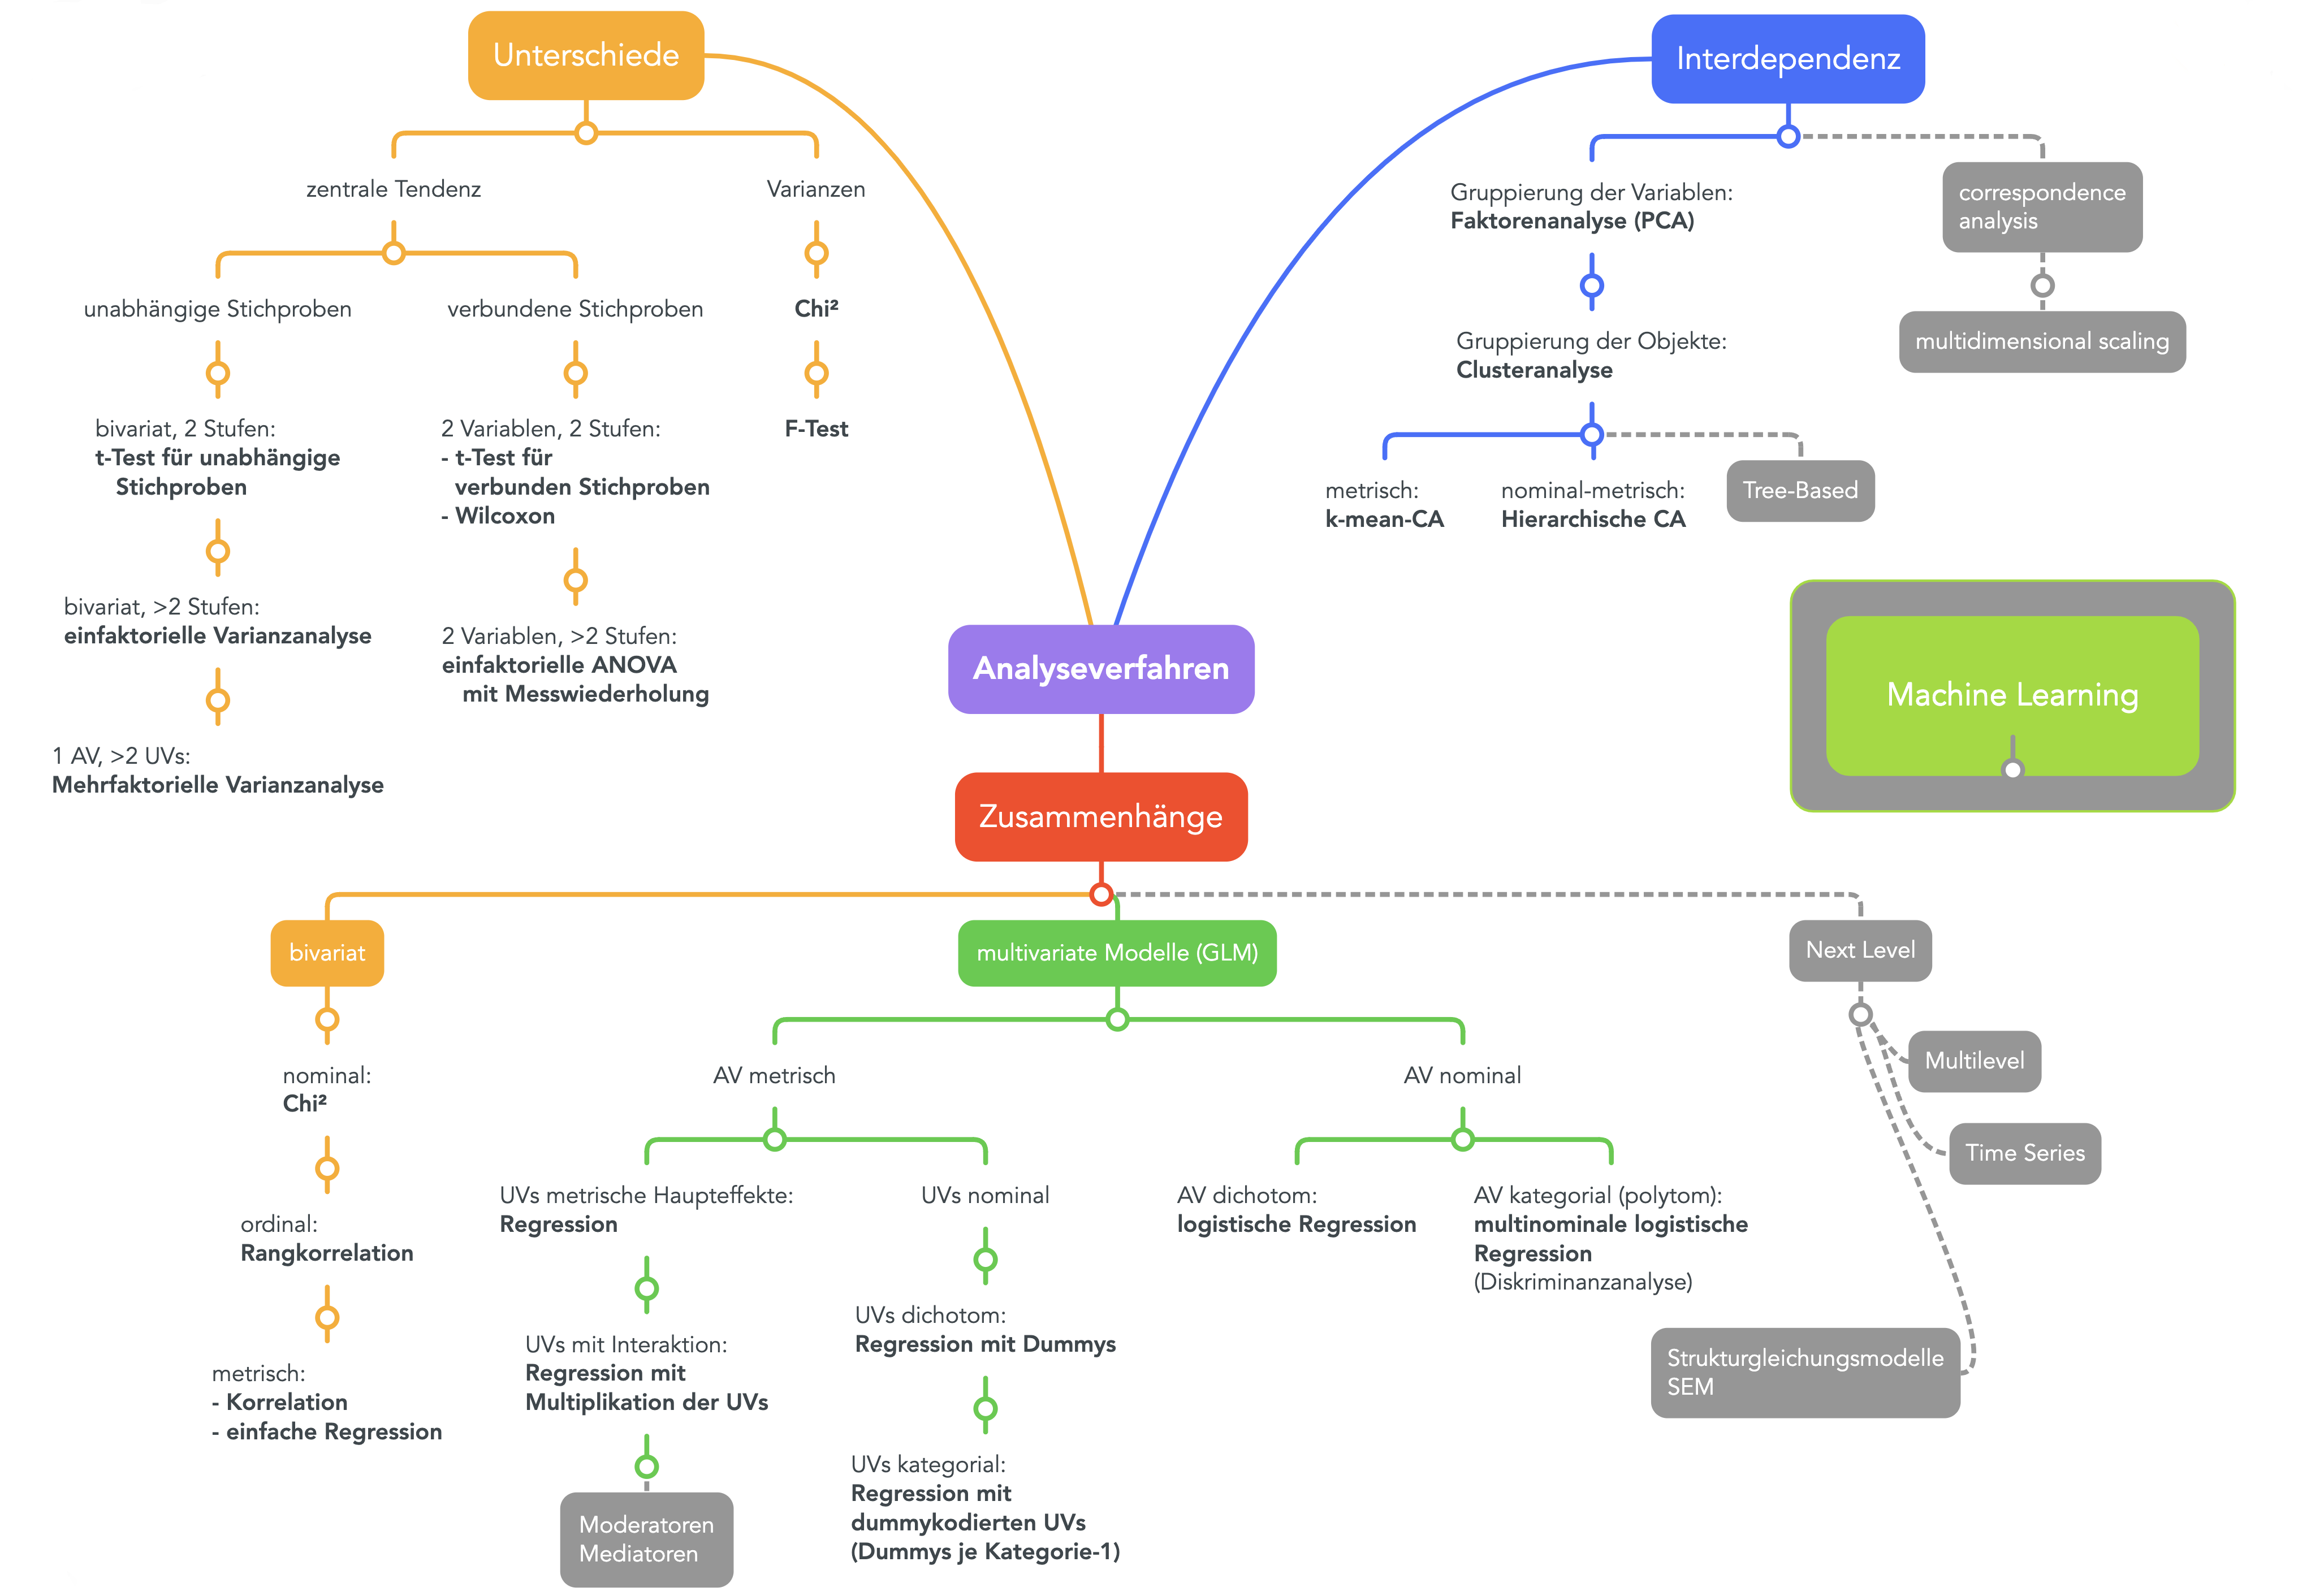
\includegraphics[width=1\textwidth,height=\textheight]{images/Analyseschema-total2.png}

}

\caption{Systematik gesamt}

\end{figure}%

\section*{Zitation dieser Seite}\label{zitation-dieser-seite}
\addcontentsline{toc}{section}{Zitation dieser Seite}

\markright{Zitation dieser Seite}

\begin{center}\rule{0.5\linewidth}{0.5pt}\end{center}

Zitation: Fretwurst, B. (2022). \emph{Statistik und Datenanalyse:
Aufbau. Begleittext zum Modul am IKMZ im HS22.}
https://www.ikmz.uzh.ch/static/methoden/Statistik-Aufbau/. Abrufdatum:
{[}aktuelles Datum{]}.

\begin{center}\rule{0.5\linewidth}{0.5pt}\end{center}

\bookmarksetup{startatroot}

\chapter{Einführung}\label{einfuxfchrung}

\section*{Der Vorlesungsmitschnitt}\label{der-vorlesungsmitschnitt}

\markright{Der Vorlesungsmitschnitt}

\section{Einleitung}\label{einleitung}

Absätze werden einfach mit einer Leerzeile getrennt. Hier finden sich
weitere Basiscs: https://quarto.org/docs/authoring/markdown-basics.html

Am Anfang war \ldots{}

Im Folgenden wird ein Video eingebettet:

\textbf{Im Tutorial schrittweise und graphisch erläutert:}

\url{https://www.youtube.com/embed/jXH1ly3Q87U}

:::

\subsection{Aufzählungen sind
einfach}\label{aufzuxe4hlungen-sind-einfach}

\begin{itemize}
\tightlist
\item
  das wird eine einfach Aufzählung mit Punkten

  \begin{itemize}
  \tightlist
  \item
    eingerückt wird eingerückt
  \item
    wird eingerückt
  \end{itemize}
\item
  oder so
\end{itemize}

Es geht auch nummeriert:

\begin{enumerate}
\def\labelenumi{\arabic{enumi}.}
\tightlist
\item
  Könnte in der Auswahlgesamtheit der wahre Wert auch 0 sein, oder ein
  anderes Vorzeichen haben?
\item
  Die Nullhypothese ist eine statistische Hypothese gegen
  Falschentscheidungen aufgrund von Zufallsziehungen.
\item
  Nullhypothesen werden anhand von bekannten Verteilungen getestet.
\end{enumerate}

\subsection{Grafiken können einfach in den
Text}\label{grafiken-kuxf6nnen-einfach-in-den-text}

\begin{figure}

\centering{

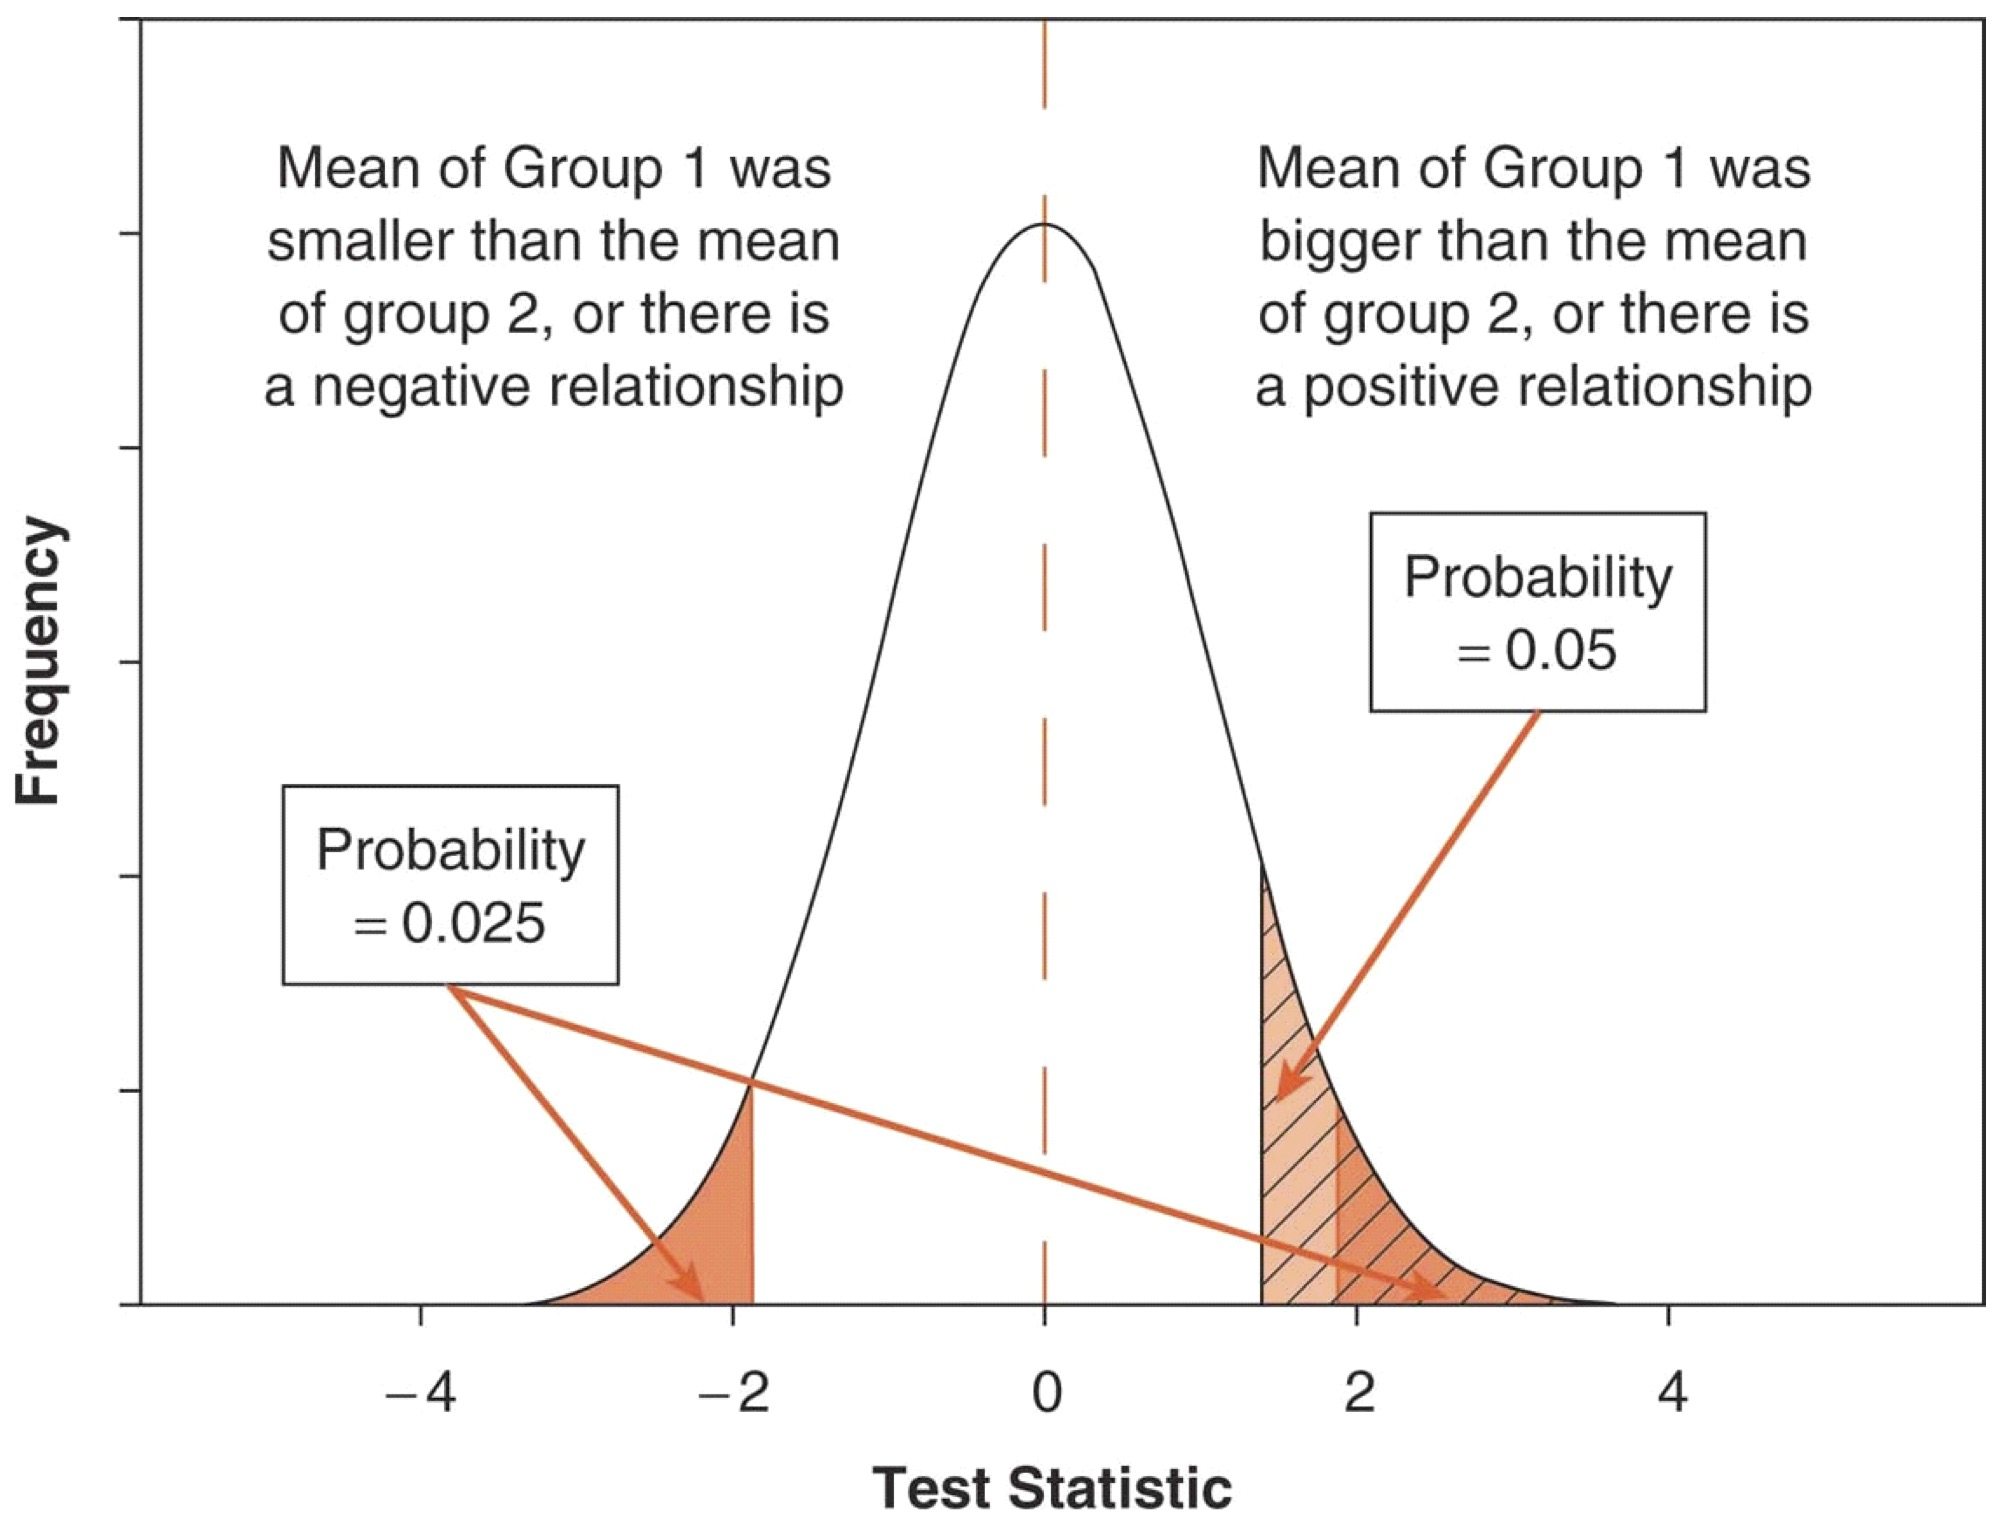
\includegraphics[width=0.8\textwidth,height=\textheight]{images/TestStat1.jpg}

}

\caption{\label{fig-Hypothesen}Hypothesentesten}

\end{figure}%

\subsection{Formeln gehen auch}\label{formeln-gehen-auch}

Die z-Transformation (auch \enquote{Standardisierung}) einer Variable
bedeutet, dass man sie so \enquote{verschiebt}, dass sie um den
Mittelwert 0 streut und zwar mit einer Standardabweichung von 1. Dazu
wird von jedem Wert \(x_i\) der Mittelwert abgezogen und diese Differenz
durch die Standardabweichung geteilt:

\begin{align}    
  z_i= & \frac{x_i-\bar{x}}{s} \label{eq:z-Transformation} 
\end{align}

Ein kleiner Einschub:

\begin{center}\rule{0.5\linewidth}{0.5pt}\end{center}

Bla, kleiner Exkurs

\begin{center}\rule{0.5\linewidth}{0.5pt}\end{center}

\begin{tcolorbox}[enhanced jigsaw, opacitybacktitle=0.6, toptitle=1mm, rightrule=.15mm, titlerule=0mm, breakable, colbacktitle=quarto-callout-important-color!10!white, colback=white, arc=.35mm, coltitle=black, bottomrule=.15mm, leftrule=.75mm, bottomtitle=1mm, colframe=quarto-callout-important-color-frame, opacityback=0, toprule=.15mm, left=2mm, title={Q\&A: Was sind eigentlich wissenschaftliche Modelle?}]

Modelle sind \ldots{}

\end{tcolorbox}


% 
\end{document}
